\newpage
\section{Rep-Tiles}

A \textbf{rep-tile}\index{rep-tile} is a polygon where several copies of
a given rep-tile fit together to make a larger, similar, version of
itself. If $2$ copies are used, we call it a \textit{rep-2-tile}, if
$3$ copies are used, we call it a \textit{rep-3-tile}, and if $n$ copies
are used, we call it a \textit{rep-n-tile}.


\begin{prob}
With a separate sheet of paper, draw and cut out:
\begin{enumerate}
\item An isosceles right triangle whose sides have lengths $1''$, $1''$, and $\sqrt{2}''$.
\item A rectangle whose sides have lengths $1''$ and $\sqrt{2}''$.
\end{enumerate}
Working with a partner, show that each of these polygons is a rep-2-tile.
\end{prob}

\begin{prob}
For each rep-tile above, compute the perimeter and area. In each case,
how does this relate to the perimeter and area of the larger polygon?
\end{prob}

\fixnote{Use Delanie's table instead, perhaps as a second investigation.  Spend some time working with the figures, computing areas and perimeters, and practicing arithmetic of radicals.  Move the summary to the second day.}


\begin{prob}
With a fresh sheet of paper, start a table:
\begin{center}
\begin{tabular}{c|c|c}
rep-$n$-tile & $\dfrac{\text{new perimeter}}{\text{old perimeter}}$ & $\dfrac{\text{new area}}{\text{old area}}$  \\
\hline\hline
 2 & $\vdots$  &  $\vdots$  \\ 
3 & $\vdots$  &  $\vdots$  \\ 
\end{tabular}
\end{center}
\end{prob}


\begin{prob}
Geometry Giorgio suggests that a rectangle whose sides have lengths
$1''$ and $4''$ is also a rep-2-tile. Is he right? If you should
happen to search the internet for other examples of rep-2-tiles, you
might find a surprise.
\end{prob}


\begin{prob}
With a separate sheet of paper, draw and cut-out:
\begin{enumerate}
\item A 30-60-90 right triangle whose shortest side has length $1''$.
\item A rectangle whose sides have lengths $1''$ and $\sqrt{3}''$.
\end{enumerate}
Working with a partner, show that each of these polygons is a rep-3-tile.
\end{prob}

\begin{prob}
For each rep-tile above, compute the perimeter and area. In each case,
how does this relate to the perimeter and area of the larger polygon?
Add this information to your table.
\end{prob}


\begin{prob}
Explain why every triangle and every parallelogram is a
rep-4-tile. Give an example of each, and compute the perimeter and
area. In both cases, compare the perimeter and area to that of the
larger polygons.
\end{prob}


%\break

\begin{prob}
With a separate sheet of graph paper, draw and cut out the following polygons:
\[
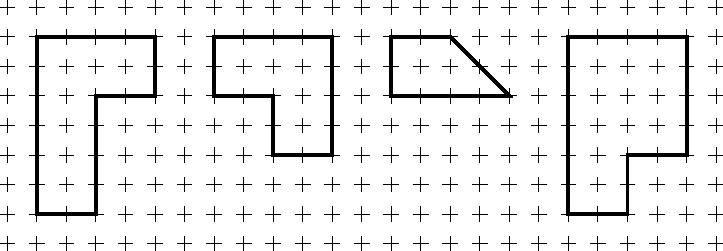
\includegraphics{../graphics/rep-4-tile1.pdf}
\]
Working with a partner, show that each of these polygons is a rep-4-tile.
\end{prob}

\begin{prob}
For each rep-tile above, compute the perimeter and area. In each case,
how does this relate to the perimeter and area of the larger polygon?
Add this information to your table.
\end{prob}


\begin{prob}
With a separate sheet of paper, trace and cut out the following
polygons:
\[
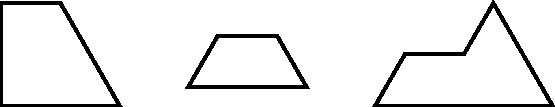
\includegraphics{../graphics/rep-4-tile2.pdf}
\]
Working with a partner, show that each of these polygons is a rep-4-tile.
\end{prob}


\begin{prob}
Explain why every rectangle whose sides have ratio $1:\sqrt{n}$ is a
rep-$n$-tile.
\end{prob}

\begin{prob}
Explain how you know that any rep-tile will tessellate the plane.
\end{prob}

\begin{prob}
Give an example of a polygon that tessellates the plane that is not a
rep-tile.
\end{prob}


\begin{prob}
Every tessellation made by rep-tiles will have \index{symmetry of
scale}\textbf{symmetry of scale}. What does it mean to have \textit{symmetry of scale}?
\end{prob}

\begin{prob}
Consider the tessellations made by rep-tiles you've seen so far. What
other symmetries do they have?
\end{prob}

\begin{prob}
Do you think you can have a tessellation that has symmetry of scale
but no other symmetries?
\end{prob}
